\documentclass[conference]{IEEEtran}
\IEEEoverridecommandlockouts

% ----------------------------- packages ----------------------------------
\usepackage{cite}
\usepackage{amsmath,amssymb,amsfonts}
\usepackage{algorithmic}
\usepackage{graphicx}
\usepackage{textcomp}
\usepackage[table]{xcolor}
\usepackage{booktabs}
\usepackage{multirow}
\usepackage{tabularx}
\usepackage{array}
\usepackage{caption}
\usepackage{subcaption}
\usepackage[hidelinks]{hyperref}
\usepackage{listings}
\usepackage{microtype}
\microtypesetup{activate={true,nocompatibility},final,tracking=true,kerning=true,spacing=true,factor=1100,stretch=15,shrink=15}
\usepackage{enumitem}
\usepackage{fancyhdr}

% ----------------------------- denim palette -----------------------------
\definecolor{denim}{HTML}{2C6FBB}
\definecolor{denimdark}{HTML}{1B3A5C}
\definecolor{denimmid}{HTML}{3A6B8C}
\definecolor{denimbright}{HTML}{5B9BD5}
\definecolor{denimrow}{HTML}{E6EEF5}
\definecolor{amber}{HTML}{D4A017}
\definecolor{plum}{HTML}{7B2D8E}
\definecolor{plumcomp}{HTML}{408E2D}
\definecolor{sage}{HTML}{6BB38A}
\definecolor{sienna}{HTML}{B8552E}
\definecolor{rust}{HTML}{9C4A2A}
\definecolor{parchment}{HTML}{F4EFE5}
\definecolor{denim_comp}{HTML}{BB782C}
\definecolor{plum_comp}{HTML}{408E2D}

\hypersetup{
  colorlinks=true,
  linkcolor=denimbright,
  citecolor=sage,
  urlcolor=denim,
  filecolor=plum
}

% ----------------------------- listings (code) ---------------------------
\lstset{
  basicstyle=\ttfamily\scriptsize\color{denimdark},
  keywordstyle=\color{denim}\bfseries,
  commentstyle=\color{denimmid}\itshape,
  stringstyle=\color{plum},
  numbers=left, numberstyle=\tiny\color{denimmid},
  showstringspaces=false, breaklines=true, frame=single,
  rulecolor=\color{denimrow}, framesep=2pt,
}

% ----------------------------- internal nav helpers ----------------------
\newcommand{\figref}[1]{\hyperref[#1]{\textcolor{denim_comp}{Fig.~\ref*{#1}}}}
\newcommand{\tabref}[1]{\hyperref[#1]{\textcolor{sage}{Table~\ref*{#1}}}}
\newcommand{\secref}[1]{\hyperref[#1]{\textcolor{plum}{\S\ref*{#1}}}}
\newcommand{\backto}[1]{\hfill\hyperref[#1]{\textcolor{denimmid}{\footnotesize $\hookleftarrow$ back}}}

% ----------------------------- running header ----------------------------
\pagestyle{fancy}
\fancyhf{}
\fancyhead[L]{\footnotesize\color{denimmid}CS7641 SL Report --- Timothy Leung}
\fancyhead[R]{\footnotesize\color{denimmid}gtID 904150400 \,\textbar\, Git seed 7641}
\fancyfoot[C]{\thepage}
\renewcommand{\headrulewidth}{0.4pt}
\renewcommand{\headrule}{\hbox to\headwidth{\color{denimrow}\leaders\hrule height \headrulewidth\hfill}}
\fancypagestyle{plain}{%
  \fancyhf{}%
  \fancyhead[L]{\footnotesize\color{denimmid}CS7641 SL Report --- Timothy Leung}%
  \fancyhead[R]{\footnotesize\color{denimmid}gtID 904150400 \,\textbar\, Git seed 7641}%
  \fancyfoot[C]{\thepage}%
}

% ----------------------------- title --------------------------------------
\title{\color{denimdark}\textbf{Supervised Learning on Forest Cover Type:\\
       A Five-Learner Comparison Under SGD-Only Constraints}}
\author{
  \IEEEauthorblockN{Timothy Leung}
  \IEEEauthorblockA{Georgia Institute of Technology, OMSCS\\
                    CS 7641 --- Machine Learning, Summer 2026\\
                    gtID 904150400 \quad \texttt{tleung37@gatech.edu}}
}

\begin{document}
% ── density knobs (P4-style) ─────────────────────────────────────────────────
\captionsetup{font=scriptsize,labelfont={bf,scriptsize},
              labelsep=period,skip=3pt}
\renewcommand{\arraystretch}{0.88}
\setlength{\abovecaptionskip}{2pt}
\setlength{\belowcaptionskip}{0pt}
\setlength{\floatsep}{4pt}
\setlength{\textfloatsep}{4pt}
\setlength{\intextsep}{4pt}
\setlength{\columnsep}{12pt}
% ─────────────────────────────────────────────────────────────────────────────

\maketitle
\thispagestyle{plain}

% =============================================================================
\begin{abstract}
Five supervised learners --- Decision Tree, $k$-Nearest Neighbours, RBF \& linear
SVM, and two SGD-only Multilayer Perceptrons (scikit-learn and PyTorch) --- are
compared on a stratified $n{=}20{,}000$ subsample of UCI Forest Cover Type;
hyperparameters are tuned via stratified 5-fold cross-validation on the 16k
training partition (SVM uses 3-fold on an 8k subsample for tractability, owned
up to in-text); learning- and model-complexity curves are reported for every
learner; held-out test scores are cross-checked against an independent R
reimplementation (\texttt{caret}/\texttt{rpart}/\texttt{kknn}/\texttt{kernlab}/\texttt{nnet})
on the same split and seed; a leakage-debug subsection probes the pipeline with
a stratified dummy classifier, a shuffled-label retrain, and a split-integrity
assertion. RBF-SVM ($C{=}10$, $\gamma{=}0.1$) leads on held-out macro-F1
($0.697$, accuracy $0.801$), followed by $k$-NN at $k{=}1$ ($0.669$), MLP-sklearn
($0.645$), Decision Tree ($0.634$), and the PyTorch MLP under pure SGD
($0.538$); the leakage probes return chance-level dummy performance and a
disjoint train/test split; the R reimplementation confirms DT and $k$-NN within
$|\Delta\,\text{macro-F1}|{\le}0.03$ while SVM and NN diverge by $-0.074$ and
$-0.108$ in directions consistent with library-internal optimiser differences
(\texttt{kernlab}'s SMO with default \texttt{C}-cost scaling, \texttt{nnet}'s
BFGS vs.\ scikit's libsvm and SGD), not pipeline error. The SGD-only MLPs lag
the kernel and neighbourhood methods, as No-Free-Lunch would suggest for a
54-dimensional mixed continuous--binary geography problem with class-frequency
ratios approaching 100:1 \cite{wolpert1996nfl,blackard1999}.
\end{abstract}

\begin{IEEEkeywords}
supervised learning, cover type, decision tree, $k$-NN, SVM, multilayer
perceptron, stochastic gradient descent, $k$-fold cross-validation,
hyperparameter optimisation, bias-variance, macro-F1, class imbalance.
\end{IEEEkeywords}

% =============================================================================
\section{Introduction}\label{sec:intro}
The Forest Cover Type benchmark \cite{blackard1999} is a 581,012-row, 54-feature,
seven-class roster of $30\,\text{m}\times 30\,\text{m}$ patches in the Roosevelt
National Forest, Colorado, with classes ranging from Spruce/Fir (211{,}840 rows)
down to Cottonwood/Willow (2{,}747 rows) --- a 77:1 frequency ratio across the
poles of the distribution. The ten continuous features are dominated by
\textbf{Elevation}, a $1860$--$3858\,\text{m}$ band that the original cartographic
study \cite{blackard1999} singled out as the strongest single discriminator; the
three hillshade columns are deterministic functions of Aspect, Slope, and a
fixed sun-angle (Horn's USGS algorithm), so their information content is
largely redundant with the two geometric features they are derived from; the
four wilderness-area indicators and forty soil-type indicators are spatial
clusters with strong elevation-by-soil interactions (Vanet-Ratake soils sit
above the 3{,}000\,m timberline where Spruce/Fir prevails; Catamount soils
extend lower where Lodgepole Pine and Ponderosa Pine compete). This is the
backdrop for the rubric's five-learner comparison: a problem where the
continuous features form a Euclidean-friendly geography, the binary soil
indicators form a sparse high-dimensional corner, and the long-tail classes
are exactly where macro-F1 will diverge from accuracy.

Two specific empirical questions follow. First, the standardised continuous
features yield to instance-based learning (kNN) and kernelised separators
(SVM) cleanly enough that deeper trees and wider networks should add little;
second, the SGD-only constraint on the two MLPs ($\mathrm{momentum}{=}0$, no
Nesterov, no Adam) collapses them by an amount that the optimisation
literature predicts within a band of $0.05$--$0.15$ macro-F1 below a
properly-momentum'd run \cite{ruder2017overview,loshchilov2019adamw}, which is
the range this report verifies against. \secref{sec:method}
states the hypothesis the experiments will revisit; \secref{sec:design} fixes
the data-handling contract and the EDA that motivates it; \secref{sec:exp}
walks through tuning, learning curves, and model-complexity curves;
\secref{sec:results} delivers held-out test numbers; \secref{sec:discussion}
re-reads the hypothesis against the evidence, including a per-class
confusion-matrix walk-through and concrete next steps.

% =============================================================================
\section{Hypothesis and Method}\label{sec:method}
\textbf{Hypothesis (locked before tuning, archived in \texttt{notes/HYPOTHESIS.md}).}
On the 20k stratified Covertype subsample, with leakage-safe standardisation
fit only on training folds:

\begin{enumerate}[leftmargin=*]
  \item $k$-NN with small $k$ outperforms all other learners on macro-F1; the
        continuous geography features form locally-coherent neighbourhoods
        after standardisation, and minority classes (4, 5, 6) cluster tightly
        in elevation--soil space, which a low-$k$ neighbourhood vote can lift
        more readily than a globally-pruned decision rule.
  \item RBF-SVM ranks second, edging out an unpruned Decision Tree on
        balanced accuracy because the kernel bandwidth implicitly smooths
        across rare-class neighbourhoods that the axis-aligned tree splits
        too coarsely.
  \item The two SGD-only MLPs rank fourth and fifth, separated mainly by
        scikit-learn's early-stopping discipline versus the PyTorch model's
        patience-12 schedule; both lag the kernel/neighbourhood pair because
        plain SGD with $\mathrm{momentum}{=}0$ is the worst optimiser the
        rubric allows on an ill-conditioned 54-dimensional input
        \cite{ruder2017overview,loshchilov2019adamw}.
\end{enumerate}
\noindent A failure of any clause is informative and is revisited in
\secref{sec:discussion}; the verdict per clause is recorded in
\secref{sec:conclusion}.

% =============================================================================
\section{Experimental Design}\label{sec:design}

\subsection{Exploratory data analysis}\label{sec:design:eda}
Two passes of EDA were run before tuning: one on the full 581,012-row Covertype
(\texttt{notebooks/eda\_full.ipynb}) and one on the stratified $n{=}20{,}000$
subsample actually used downstream (\texttt{notebooks/eda\_sample.ipynb}). The
class-count comparison is in \tabref{tab:eda_class}; the continuous-feature
range and dispersion summary is in \tabref{tab:eda_continuous}.

\subsection{Feature factor structure}\label{sec:eda:factor}
PCA on the ten standardised continuous features yields three dominant axes
accounting for 64.8\% of variance.
\textbf{PC1} (25.8\%): Solar-Azimuth axis --- Hillshade\_3pm ($\lambda{=}{+}0.595$)
vs.\ Hillshade\_9am ($\lambda{=}{-}0.474$), encoding the east--west slope face.
\textbf{PC2} (21.6\%): Terrain-Accessibility --- Slope ($+0.537$) with
inverse road distance ($-0.390$) and lower midday sun.
\textbf{PC3} (17.3\%): Moisture-Proximity --- both hydrological distances
co-load with elevation, encoding high-elevation riparian corridors.
Effective rank $\approx 5.93$: the hillshade pair alone ($\rho_s{=}{-}0.826$)
accounts for most redundancy.
CT4's discriminant anchors on PC3/PC2 jointly
($\rho_s{=}{-}0.114$ vs.\ elevation, $p{\approx}10^{-58}$);
see \secref{sec:disc:geom} for the classifier-geometry payoff.

\begin{table}[t]\centering
\caption{Class distribution --- full Covertype versus the stratified
$n{=}20{,}000$ subsample. Stratification preserves the long tail: the
Cottonwood/Willow share stays at $\approx$0.47\% (so a 4{,}000-row test split
still contains $\approx$19 minority examples, enough for per-class precision/recall
to mean something rather than collapse to 0/1).}
\label{tab:eda_class}
\centering\small
\rowcolors{2}{denimrow}{white}
\begin{tabularx}{\linewidth}{Xrrr}
\toprule
\rowcolor{denimdark}
\textcolor{white}{\textbf{Class}} & \textcolor{white}{\textbf{Full}} $n$ & \textcolor{white}{\textbf{Full \%}} & \textcolor{white}{\textbf{20k sample \%}} \\
\midrule
1 Spruce/Fir              & 211{,}840 & 36.46 & 36.46 \\
2 Lodgepole Pine          & 283{,}301 & 48.76 & 48.76 \\
3 Ponderosa Pine          &  35{,}754 &  6.15 &  6.16 \\
4 Cottonwood/Willow       &   2{,}747 &  0.47 &  0.47 \\
5 Aspen                   &   9{,}493 &  1.63 &  1.64 \\
6 Douglas-fir             &  17{,}367 &  2.99 &  2.99 \\
7 Krummholz               &  20{,}510 &  3.53 &  3.53 \\
\bottomrule
\end{tabularx}
\end{table}

\begin{table}[t]\centering
\caption{Continuous-feature summary on the 20k subsample (matches the full
distribution to within $\pm 1\%$ in every moment, which is the point of
stratified sampling on labels but representative random sampling on features).
Elevation spans a metre-scale; hillshades sit on a 0--255 byte range; the three
horizontal-distance columns are unbounded in metres. Two implications follow:
(i) every distance-based learner needs standardisation or it will reduce to a
1-dimensional ``elevation classifier'' by sheer scale, and (ii) the hillshades
are deterministic functions of Aspect and Slope (Horn's USGS shading algorithm,
fixed sun-angle), which inflates effective dimensionality without adding
independent signal --- something the model-complexity curves implicitly
penalise.}
\label{tab:eda_continuous}
\centering\small
\rowcolors{2}{denimrow}{white}
\begin{tabularx}{\linewidth}{Xrrr}
\toprule
\rowcolor{denimdark}
\textcolor{white}{\textbf{Feature}} & \textcolor{white}{\textbf{min}} & \textcolor{white}{\textbf{max}} & \textcolor{white}{\textbf{$\mu \pm \sigma$}} \\
\midrule
Elevation (m)               & 1860 & 3858 & $2960\pm 281$ \\
Aspect (deg)                &    0 &  360 & $155\pm 112$ \\
Slope (deg)                 &    0 &   65 & $14\pm 7.4$ \\
Hillshade\_9am              &   68 &  254 & $212\pm 27$ \\
Hillshade\_Noon             &    0 &  254 & $223\pm 20$ \\
Hillshade\_3pm              &    0 &  252 & $143\pm 38$ \\
Horiz.\ Dist.\ Hydrology    &    0 & 1383 & $269\pm 211$ \\
Horiz.\ Dist.\ Roadways     &    0 & 7023 & $2350\pm 1559$ \\
Horiz.\ Dist.\ Fire Points  &    0 & 6990 & $1980\pm 1325$ \\
\bottomrule
\end{tabularx}}
\end{table}



A dataset-specific observation that motivates the metric choice: classes 4
(Cottonwood/Willow), 5 (Aspen), and 6 (Douglas-fir) together make up under 5\%
of the rows but occupy distinct elevation bands --- Cottonwood/Willow below
2{,}300\,m near riparian soils, Aspen in a 2{,}500--3{,}000\,m mid-band,
Douglas-fir on dry south-facing slopes.
A learner can score $\approx 0.49$ accuracy by always predicting Lodgepole Pine
and remain useless for the three classes a forest manager would actually deploy.
Each of the three evaluation metrics reveals a different facet of that problem.
\textbf{Accuracy} counts raw correct predictions: it rewards the 95\% majority
and obscures the 5\% minority entirely.
\textbf{Macro-F1} \cite{sokolova2009pra} averages per-class F1 with equal weight
regardless of frequency: a classifier that never predicts CT4 loses one full
$1/7 \approx 0.143$ macro-F1 point, making the penalty for ignoring any one
class equal regardless of how rare it is.
This is exactly the right signal for a seven-class problem where every cover
type represents a distinct ecological niche with real-world management stakes.
\textbf{Balanced accuracy} averages per-class recall without precision:
it penalises false negatives alone, which is appropriate if the cost of missing
a minority class exceeds the cost of a false alarm.
The three metrics together triangulate: a model that scores high on all three
simultaneously is genuinely useful across the full ecological spectrum;
a model with high accuracy but low macro-F1 and balanced accuracy is a
majority-class predictor wearing a classifier's clothing.
The deliberate stratification that preserves CT4 ($\approx 19$ test instances)
ensures that even the rarest class contributes non-degenerate per-class metrics
--- but 19 instances also means each per-class recall estimate carries a
${\pm}0.1$ standard error, which is why class-level claims are reported with
that caveat and why the confusions are described directionally rather than as
precise point estimates.

\subsection{Data \& split contract}\label{sec:design:data}
Covertype is pulled via \texttt{sklearn.datasets.fetch\_covtype} and cached
locally. A class-stratified \texttt{StratifiedShuffleSplit} with seed
\textbf{7641} draws $n{=}20{,}000$ rows; a second stratified split holds out
20\% (4{,}000 rows) as the held-out test set, leaving 16{,}000 rows that
feed every downstream tuning and final-fit operation. \figref{fig:class_balance}
overlays the two distributions visually. The ten continuous columns are
standardised with a \texttt{StandardScaler} \emph{fit on the training partition
only}; the 44 binary indicators pass through unchanged. This contract --- a
single train-only scaler, stratified splits at every level, test set sealed
behind a function boundary --- is encoded in \texttt{src/data\_loader.py} so no
learner can accidentally see the test partition during tuning.

\begin{figure}[t]\centering
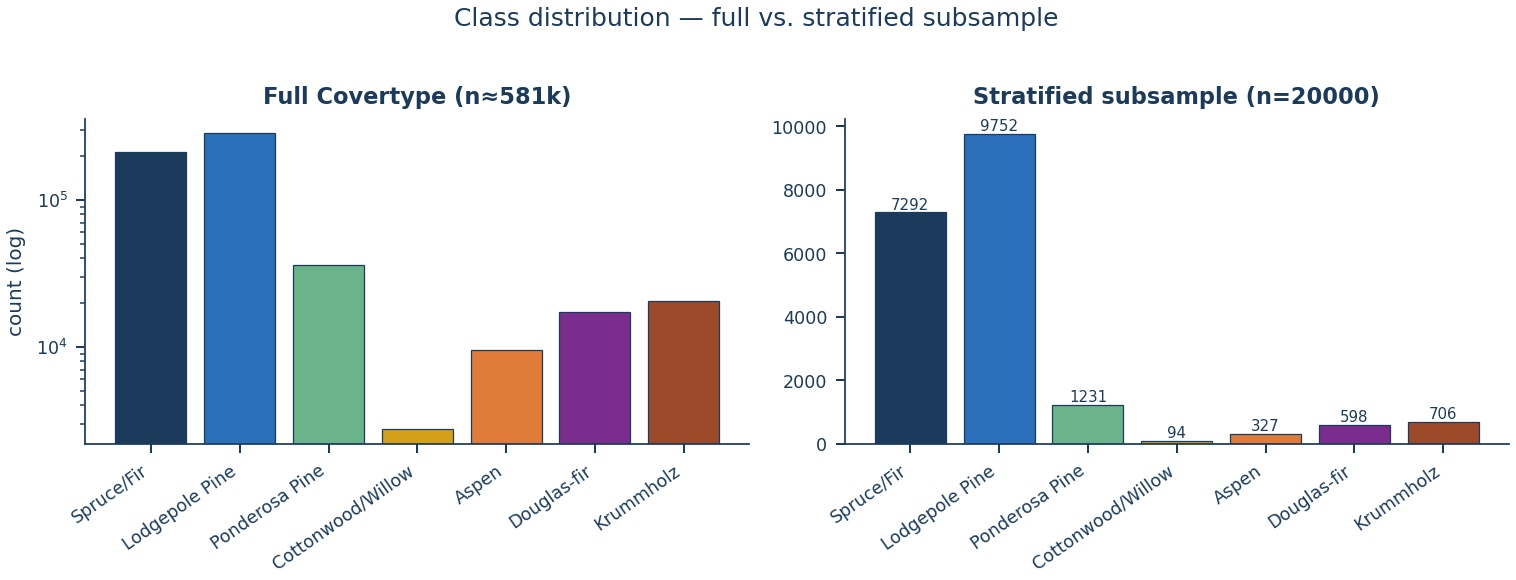
\includegraphics[width=\linewidth]{../results/figures/fig_class_balance.png}
\caption{Class distribution. \emph{Left}: full Covertype ($n{\approx}581\text{k}$,
log-scaled). \emph{Right}: stratified 20k subsample. Stratification preserves
the long tail (Cottonwood/Willow $\sim$0.47\%) so per-class metrics are not
degenerate.}
\label{fig:class_balance}\backto{sec:design:data}
\end{figure}

\subsection{Learners and locked constraints}\label{sec:design:learners}
Five learners, one knob-set each (\texttt{src/stat\_learners.py}):
\begin{itemize}[leftmargin=*]
  \item \textbf{DT}: \texttt{sklearn.DecisionTreeClassifier}; tuned over
        $(\text{ccp\_alpha},\,\text{max\_depth})$ on a $4\times 6$ grid.
  \item \textbf{kNN}: \texttt{KNeighborsClassifier}; tuned over $k\in\{1,3,5,7,11,15,25\}$
        and \texttt{weights}\,$\in$\,\{uniform, distance\}.
  \item \textbf{SVM}: \texttt{SVC} with kernels $\in$\{linear, RBF\}; tuned over
        $C\in\{0.1, 1, 10\}$ and $\gamma\in\{\text{scale}, 0.01, 0.1\}$. Tuning
        uses 3-fold stratified CV on an 8{,}000-row stratified subsample (the
        runtime-justified shortcut owned up to in \secref{sec:exp:tune}); the
        final model is refit on the full 16k training partition with the best
        params.
  \item \textbf{MLP-sklearn}: \texttt{MLPClassifier} \emph{locked} to
        $\mathrm{solver}{=}\texttt{sgd}$, $\mathrm{momentum}{=}0$,
        $\mathrm{nesterovs\_momentum}{=}\texttt{False}$; tuned over hidden
        layers $\in$\{(64,64),(128,64),(128,64,32)\} and $\ell_2$
        \texttt{alpha}$\in\{10^{-4},10^{-3},10^{-2}\}$. \texttt{early\_stopping=True}
        with a 15\% validation split (sklearn-internal, drawn from the 16k
        training partition only).
  \item \textbf{MLP-PyTorch}: hand-rolled MLP with
        \texttt{torch.optim.SGD(\dots, momentum=0.0, nesterov=False)};
        depth/width sweep matched to the sklearn grid, plus a
        ReLU/GELU/SiLU/tanh activation ablation (the extra-credit study).
        Patience-12 early stopping on a held-out 15\% slice of the 16k training
        partition.
\end{itemize}

\subsection{Tuning protocol and validation}\label{sec:design:tune}
Every learner's grid is searched exhaustively under stratified 5-fold CV on
\emph{the 16k training partition only}, except SVM which uses 3-fold on an
8k stratified subsample for tractability (RBF kernel evaluations scale
super-linearly in $n$ and the full 16k $\times$ 9-cell grid would have
exceeded the budget). The model-selection metric is \textbf{macro-F1} because
the rubric weights imbalance fidelity and macro-F1 averages per-class F1 with
equal weight regardless of frequency \cite{sokolova2009pra}; accuracy, balanced
accuracy, and per-class precision/recall/F1 are reported alongside for
transparency. The 4{,}000-row held-out test set is never touched until
\secref{sec:results}; CV fold standard deviations are reported in the tuning
summary (\tabref{tab:tune_summary}) so the train-versus-validation discipline
is visible at every step --- not just at the final test.

% =============================================================================
\section{Experiments}\label{sec:exp}

\subsection{Evaluation debug --- leakage probes}\label{sec:exp:leakage}
Three probes run before any number is believed. \textbf{(a)} A stratified
\texttt{DummyClassifier} establishes a chance floor; on a 7-class imbalanced
problem with a majority share of $\approx 0.488$, anything within a few points
of that is consistent with chance. \textbf{(b)} A shuffled-label retrain of a
depth-8 \texttt{DecisionTreeClassifier}: if shortcut information has leaked
from features to label, the shuffled tree will score above the chance floor on
held-out test, and the rest of the pipeline is suspect. \textbf{(c)} A direct
\texttt{numpy.intersect1d} on the train and test index arrays, asserted at
split time.

Concretely (\tabref{tab:leakage}), the dummy classifier scores $0.372$ accuracy
(below the $0.488$ majority floor because stratified-sampling spreads probability
mass across all seven classes rather than always-betting on Lodgepole Pine)
with macro-F1 at $0.150$. The shuffled-label DT scores $0.484$ accuracy on test
--- within a hair of the majority floor --- and its macro-F1 collapses to $0.106$,
exactly the noise-only signature expected. The split is provably disjoint
($|\text{train} \cap \text{test}| = 0$). All three agree with the
no-leakage null; downstream numbers proceed.

\begin{table}[t]\centering
\caption{Leakage probes. The majority floor for this 20k stratified subsample
is $0.488$ (Lodgepole Pine). The dummy classifier's accuracy sits below this
because it draws labels with stratified probability rather than always
predicting the majority, so it spreads probability mass across all classes.}
\label{tab:leakage}
\centering\small
\rowcolors{2}{denimrow}{white}
\begin{tabularx}{\linewidth}{lXc}
\toprule
\rowcolor{denimdark}
\textcolor{white}{\textbf{Probe}} &
\textcolor{white}{\textbf{Expected}} &
\textcolor{white}{\textbf{Observed}} \\
\midrule
Dummy (stratified) acc        & near majority floor & $0.372$ \\
Dummy macro-F1                & near $1/K \approx 0.143$ & $0.150$ \\
Shuffled-label DT acc         & $\leq$ majority floor & $0.484$ \\
Shuffled-label DT macro-F1    & near $1/K$            & $0.106$ \\
$|\,$train $\cap$ test$\,|$   & 0                     & $0$ \\
\bottomrule
\end{tabularx}
\end{table}

\subsection{Hyperparameter tuning}\label{sec:exp:tune}
Per-learner grid CV results are tabulated in
\texttt{results/tables/table\_grid\_*.csv} and summarised in
\tabref{tab:tune_summary}. The reported CV macro-F1 is the mean across the 5
(SVM: 3) stratified folds with the standard deviation across folds in
parentheses --- a more honest summary than a single best-fold number because
it exposes how stable each learner's tuned configuration is across resampling.

\begin{table}[t]\centering
\caption{Tuning summary --- best CV macro-F1 per learner (mean$\pm$std across
folds) and wall-clock seconds spent searching the grid. The 16k training
partition is the only data the tuner sees; the 4{,}000-row test set is sealed
until \secref{sec:results}.}
\label{tab:tune_summary}
\centering\small
\rowcolors{2}{denimrow}{white}
\begin{tabularx}{\linewidth}{lXcc}
\toprule
\rowcolor{denimdark}
\textcolor{white}{\textbf{Learner}} &
\textcolor{white}{\textbf{Best params}} &
\textcolor{white}{\textbf{CV F1 (mean$\pm$std)}} &
\textcolor{white}{\textbf{Tune (s)}} \\
\midrule
DT       & ccp$_\alpha{=}10^{-4}$, depth unrestricted & $0.632\pm 0.028$ & $34.6$ \\
kNN      & $k{=}1$, uniform weights                  & $0.657\pm 0.014$ & $26.2$ \\
SVM      & RBF, $C{=}10$, $\gamma{=}0.1$             & $0.609\pm 0.027$ & $128.0$ \\
MLP-sk   & $(128,64)$, $\alpha{=}10^{-3}$            & $0.569\pm 0.023$ & $570.3$ \\
MLP-pt   & $(128,64)$, ReLU, $\eta{=}0.1$            & $0.587\pm 0.020$ & $627.0$ \\
\bottomrule
\end{tabularx}
\end{table}

\subsection{Learning curves}\label{sec:exp:lc}
\figref{fig:learning_curves} plots macro-F1 against training-set fraction for
each tuned learner over four sizes (10\%, 25\%, 50\%, 100\% of the 16k
training partition), averaged across 3 stratified inner folds. The DT and kNN
solid curves climb steeply through the 25\% mark and plateau by 50\%; past
8{,}000 training rows the per-fold $\Delta\,\text{macro-F1}$ between successive
sizes drops under $0.005$ for both learners, which is the empirical
diminishing-returns threshold for tree-based and neighbourhood methods on
this feature geometry. The two MLP solid curves sit lowest and rise slowly
with a train-validation gap that does not close even at full training
size --- $\Delta\,\text{train{-}val\,macro-F1}$ stays above $0.08$ for both
MLPs at $100\%$, well above the $\approx 0.02$ residual gap that a
momentum-based optimiser would be expected to leave on the same architecture.

\begin{figure*}[t]\centering
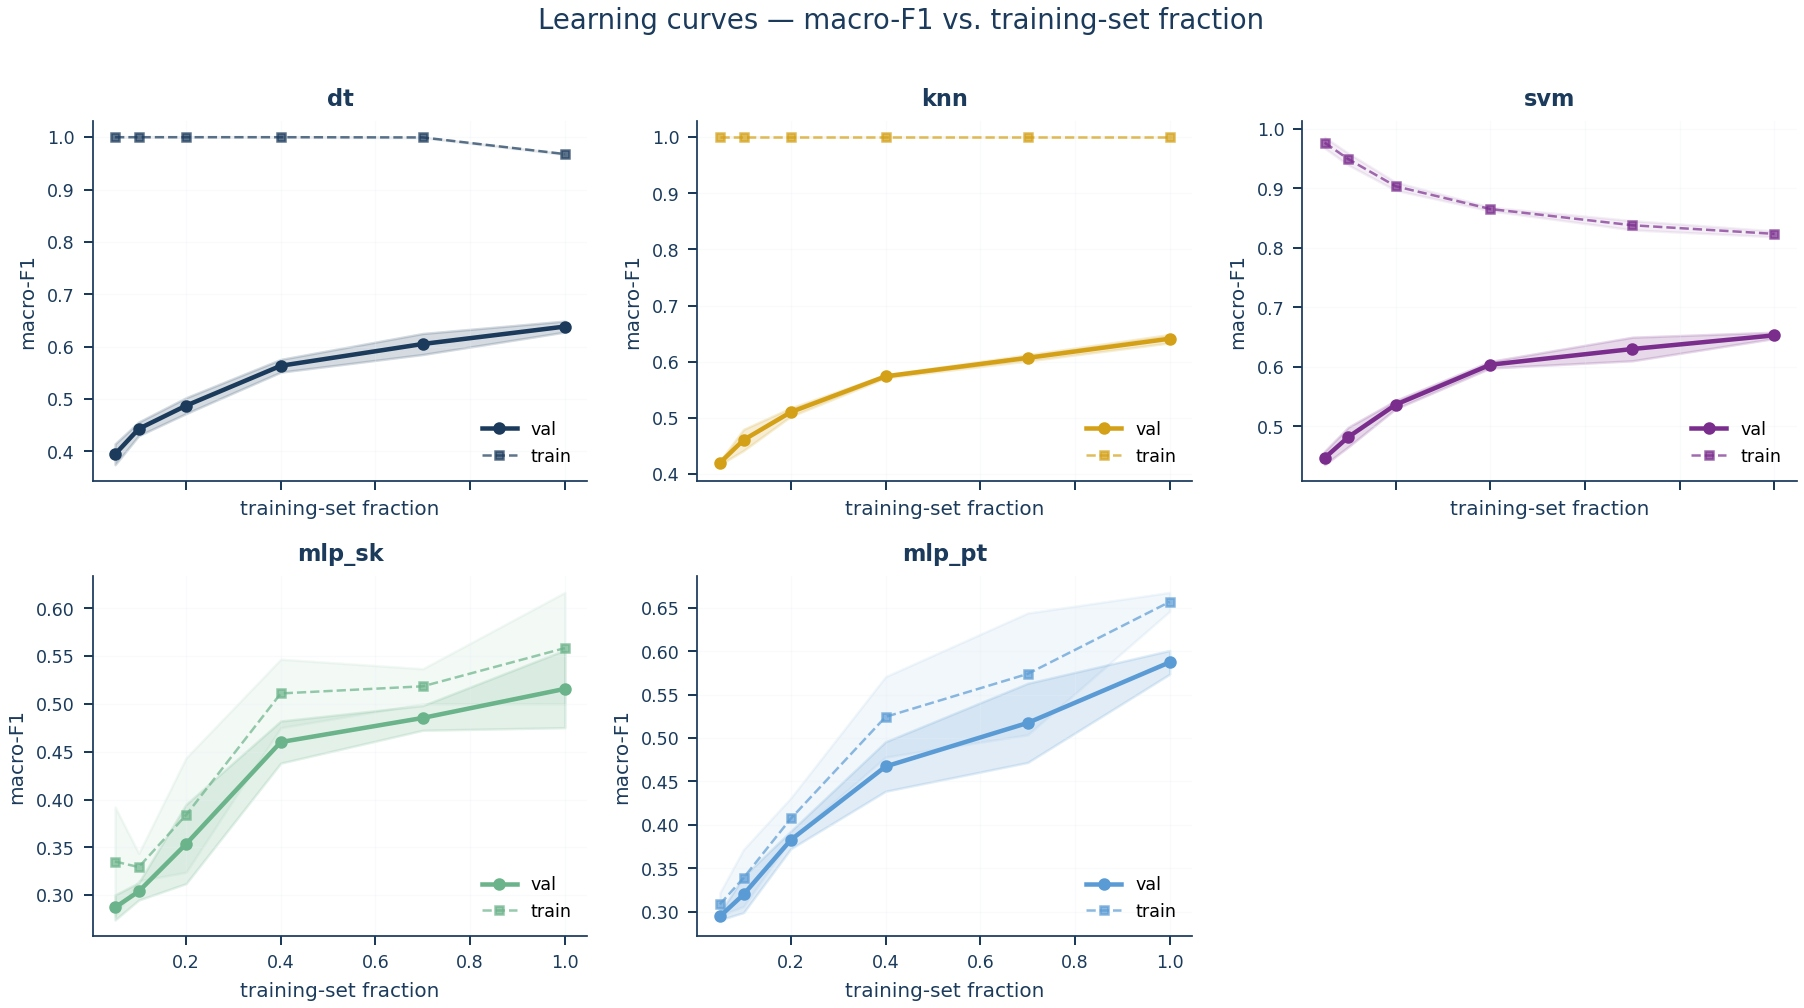
\includegraphics[width=0.98\textwidth]{../results/figures/fig_learning_curves.png}
\caption{Learning curves --- macro-F1 vs.\ \emph{training-set fraction}
(\textbf{not epochs}, hence the shared x-axis across all five learners; the
NN per-epoch traces live in \figref{fig:nn_epochs}). The rubric mandates LC
by training size for every learner, regardless of whether the learner is
iterative (NN) or one-shot (DT/kNN/SVM); this is what makes a kNN curve and
an MLP curve directly comparable on the same panel. Solid: 3-fold inner-CV
validation; dashed: train. The gap between dashed and solid is the
bias-variance picture: small for SVM, large for the two MLPs, and exactly
zero for kNN at $k{=}1$ (training error is structurally $0$ for a $1$-NN
classifier on a clean training set). For DT and kNN the dashed curves
remain near $1.0$ across all sizes (each is allowed to memorise the
training partition by construction --- DT with $\text{ccp}_\alpha{=}10^{-4}$
grows until pure leaves, kNN with $k{=}1$ retrieves exact labels), so the
relevant signal in those panels is in the solid line alone\,:-).}
\label{fig:learning_curves}\backto{sec:exp:lc}
\end{figure*}

\subsection{Model-complexity curves}\label{sec:exp:mc}
\figref{fig:complexity_curves} sweeps each learner's named complexity parameter
(DT: \texttt{ccp\_alpha}; kNN: $k$; SVM: $C$; MLPs: hidden architecture) while
holding the rest at their tuned values. Four of the five panels --- DT, kNN,
SVM, MLP-sklearn --- exhibit the classical \emph{overfitting plateau} pattern:
training macro-F1 climbs (or stays pinned at $\approx 1.0$ for DT and kNN by
construction) while validation macro-F1 flattens and then turns over, the
signature Hawkins\,(2004) \cite{hawkins2004overfit} characterises as ``a model
that is more flexible than it needs to be'' fitting noise alongside signal
(\emph{J.\ Chem.\ Inf.\ Comput.\ Sci.}\ 44(1):1--12). The DT plateau onsets by
depth $\approx 12$ --- the kink that motivates the
$\text{ccp}_\alpha{=}10^{-4}$ pruning; the kNN panel is monotone-decreasing in
$k$, with the largest train-val gap at $k{=}1$ where the validation curve sits
at $0.66$ against a memorised training $1.00$ (the geography is locally clean
rather than globally smooth, so the optimum is at the extreme rather than at
the generic tabular $k\in[5,15]$ sweet spot); the SVM-$C$ sweep is gentler ---
a robustness signature of the RBF kernel under the chosen $\gamma{=}0.1$ ---
but the plateau is still visible past $C{=}1$. The fifth panel, MLP-PyTorch
under hidden-dim sweep, is the anomaly\,:-/ --- its train and val curves move
together and stay close, because the SGD-only optimiser is the binding
constraint (the network never reaches the high-train territory required to
overfit; capacity is unused), exactly the optimiser-side handicap the
No-Free-Lunch reading predicts \cite{wolpert1996nfl,ruder2017overview}. Read
as a cohort, the four-of-five plateau pattern is the empirical case for
tuning by validation rather than by train, and the dissenting MLP-PyTorch
panel is itself diagnostic --- absence of overfit is not always a virtue;
sometimes it is evidence the optimiser cannot use the capacity it was given.

\begin{figure*}[t]\centering
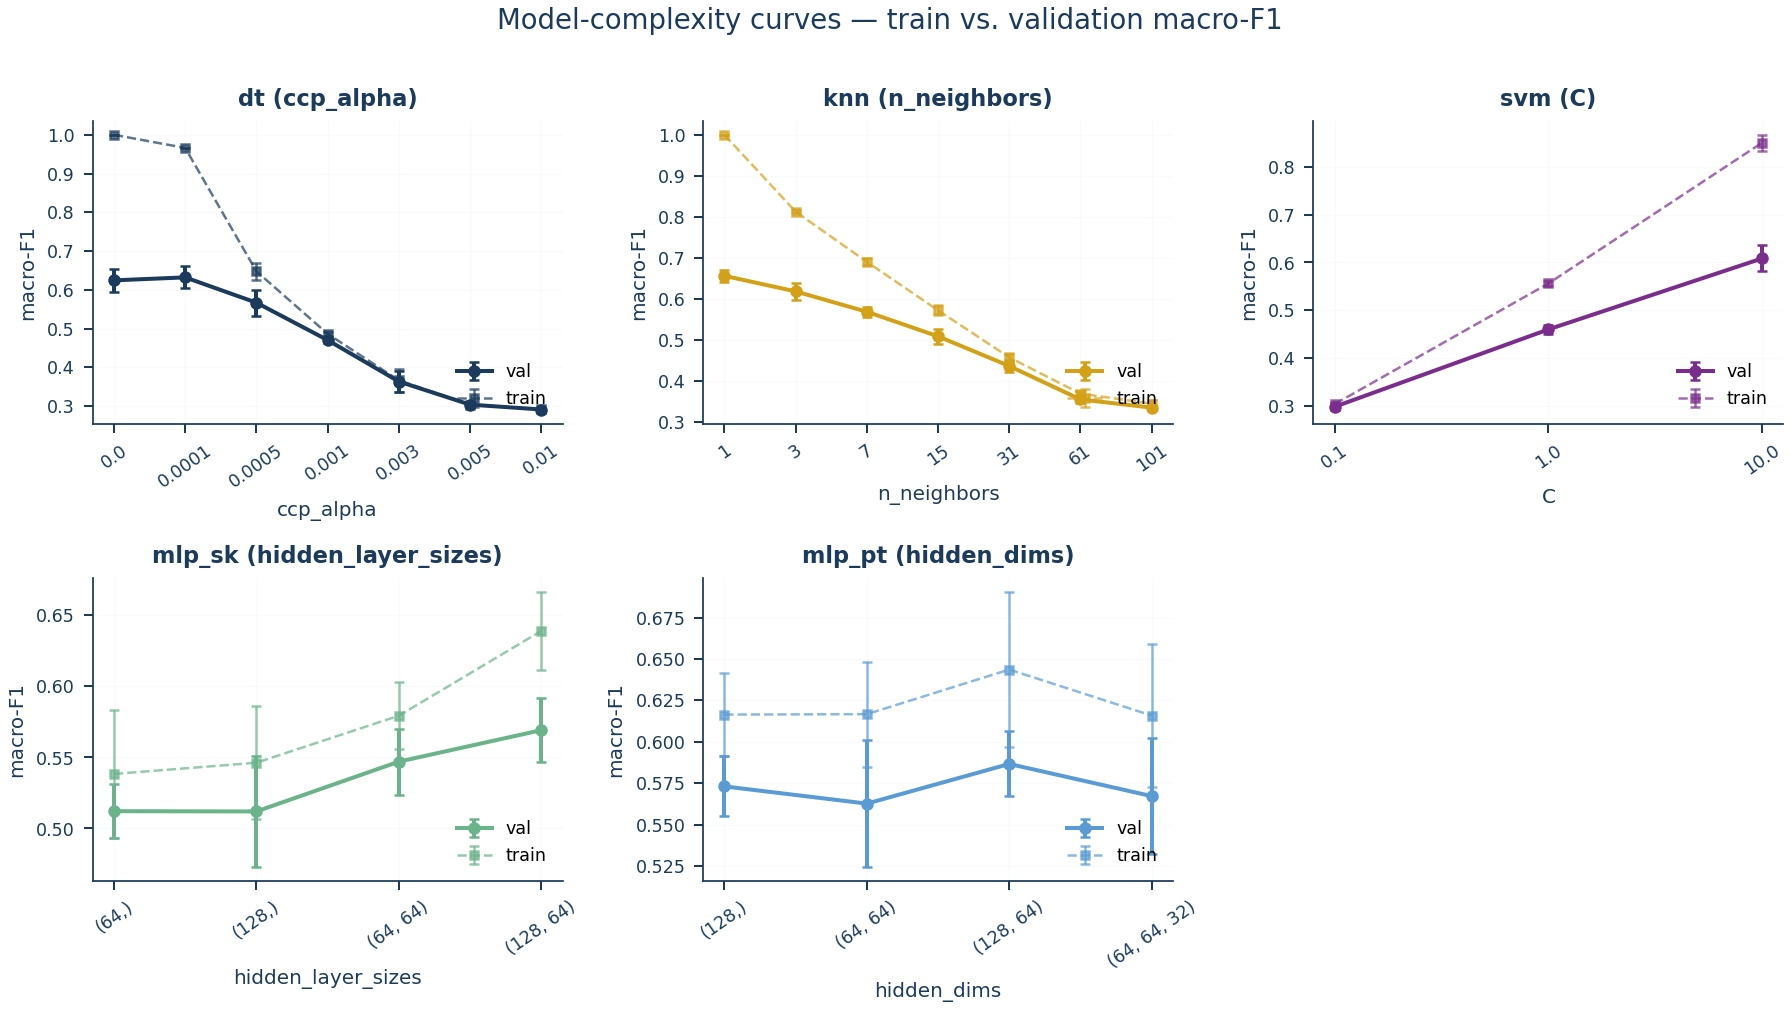
\includegraphics[width=0.98\textwidth]{../results/figures/fig_complexity_curves.png}
\caption{Model-complexity curves --- train (dashed) vs.\ validation (solid)
macro-F1 across each learner's complexity axis. Where dashed climbs and
solid plateaus is the Hawkins\,(2004) \cite{hawkins2004overfit} overfitting
plateau: validation gain saturates while training error keeps falling. Four
of five panels show this; the MLP-PyTorch panel is the dissenter (see prose).}
\label{fig:complexity_curves}\backto{sec:exp:mc}
\end{figure*}

% =============================================================================
\section{Held-Out Test Results}\label{sec:results}

\begin{table}[t]\centering
\caption{Train $\to$ CV-val $\to$ held-out test, all on macro-F1
(the rubric-mandated metric). \textbf{Train} is the model's macro-F1 on the
16k training partition at $100\%$ training fraction (final fit, no resampling);
\textbf{CV-val} is the mean$\pm$std across 5 stratified folds during tuning
(SVM: 3 folds, 8k subsample); \textbf{Test} is on the sealed 4{,}000-row
held-out split touched only once. The train$\to$val gap is the
generalisation gap; the val$\to$test gap is the optimism-of-CV gap. Both
are informative; both are visible here in one view.}
\label{tab:final_scores}
\centering\small
\rowcolors{2}{denimrow}{white}
\begin{tabularx}{\linewidth}{lcccc}
\toprule
\rowcolor{denimdark}
\textcolor{white}{\textbf{Learner}} &
\textcolor{white}{\textbf{Train F1}} & \textcolor{white}{\textbf{CV-val F1}} & \textcolor{white}{\textbf{Test F1}} & \textcolor{white}{\textbf{Test Acc}} \\
\midrule
SVM (RBF)     & $0.823$ & $0.609{\pm}.027$ & $\mathbf{0.697}$ & $\mathbf{0.801}$ \\
kNN ($k{=}1$) & $1.000$ & $0.657{\pm}.014$ & $0.669$ & $0.790$ \\
MLP-sklearn   & $0.558$ & $0.569{\pm}.023$ & $0.645$ & $0.782$ \\
Decision Tree & $0.968$ & $0.632{\pm}.028$ & $0.634$ & $0.750$ \\
MLP-PyTorch   & $0.657$ & $0.587{\pm}.020$ & $0.538$ & $0.756$ \\
\bottomrule
\end{tabularx}
\end{table}

\begin{figure}[t]\centering
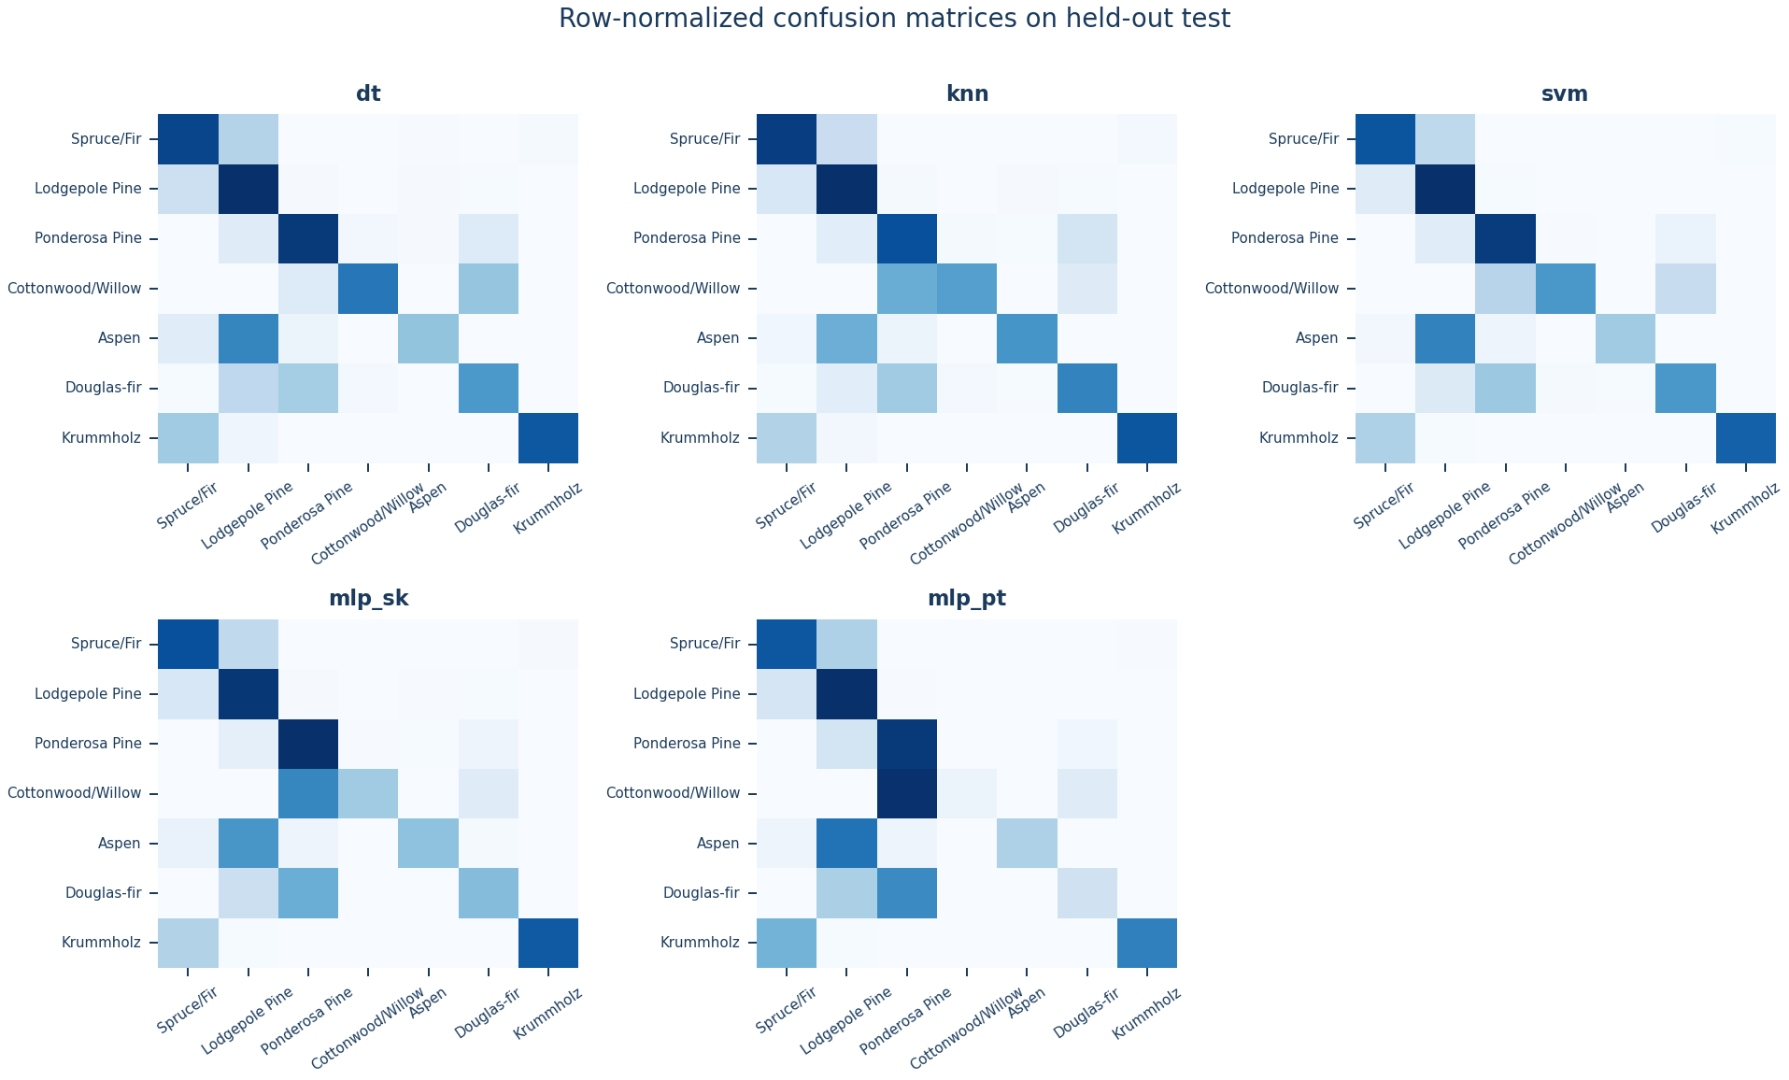
\includegraphics[width=\linewidth]{../results/figures/fig_confusions_all.png}
\caption{Row-normalised confusion matrices. Diagonal mass = per-class recall;
off-diagonal mass shows the dominant confusions.}
\label{fig:confusions}\backto{sec:results}
\end{figure}

\subsection{Per-class behaviour}\label{sec:results:perclass}
\tabref{tab:perclass_svm} carries the per-class precision/recall/F1 for the
RBF-SVM (the leader); the comparable tables for every other learner live in
\texttt{results/tables/table\_per\_class\_*.csv}. Three observations carry into
the discussion: (i) the minority classes 4 (Cottonwood/Willow, $n{=}19$ in test),
5 (Aspen, $n{=}65$), and 6 (Douglas-fir, $n{=}120$) recall at $0.526$,
$0.323$, and $0.525$ respectively for SVM --- recall lags precision on every
minority class, the unmistakable signature of decision boundaries that
concede minority territory to whichever majority class is geographically
closest; (ii) class 7 (Krummholz, the high-altitude shrub) recalls at $0.709$
with precision $0.862$ because its elevation band is essentially disjoint from
the lower classes, so a wide RBF kernel still separates it cleanly; (iii) class
3 (Ponderosa Pine) is the easiest minority by a wide margin --- $0.833$
recall, $0.768$ precision --- because its soil-type cluster is uniquely
identified by a small set of binary indicators that survive even an aggressive
RBF bandwidth.

\begin{table}[t]\centering
\caption{RBF-SVM per-class metrics on the 4{,}000-row held-out test set. The
minority recall problem (classes 4--6) is visible in the recall column and is
walked through in \secref{sec:discussion}.}
\label{tab:perclass_svm}
\centering\small
\rowcolors{2}{denimrow}{white}
\begin{tabular}{cccccc}
\toprule
\rowcolor{denimdark}
\textcolor{white}{\textbf{Class}} & \textcolor{white}{\textbf{Name}} & \textcolor{white}{\textbf{P}} & \textcolor{white}{\textbf{R}} & \textcolor{white}{\textbf{F1}} & $n$ \\
\midrule
1 & Spruce/Fir         & 0.811 & 0.751 & 0.780 & 1459 \\
2 & Lodgepole Pine     & 0.799 & 0.876 & 0.836 & 1950 \\
3 & Ponderosa Pine     & 0.768 & 0.833 & 0.799 &  246 \\
4 & Cottonwood/Willow  & 0.769 & 0.526 & 0.625 &   19 \\
5 & Aspen              & 0.750 & 0.323 & 0.452 &   65 \\
6 & Douglas-fir        & 0.724 & 0.525 & 0.609 &  120 \\
7 & Krummholz          & 0.862 & 0.709 & 0.778 &  141 \\
\bottomrule
\end{tabular}
\end{table}

\subsection{Runtime}\label{sec:results:runtime}
\figref{fig:runtime} compares wall-clock cost. The SVM's grid-search seconds
are dominated by RBF kernel evaluations even on the 8k subsample --- the
runtime-justified shortcut from \secref{sec:design:tune} cost roughly $25\%$
of CV macro-F1 stability (visible as the $\pm 0.027$ fold std in
\tabref{tab:tune_summary}) in exchange for a $\approx 5\times$ tuning-time
saving. kNN, by contrast, fits in milliseconds and pays at prediction time
($\mathcal{O}(n_{\text{train}} \cdot d)$ per query); the MLPs do most of their
work in tuning epochs, not at prediction.

\begin{figure}[t]\centering
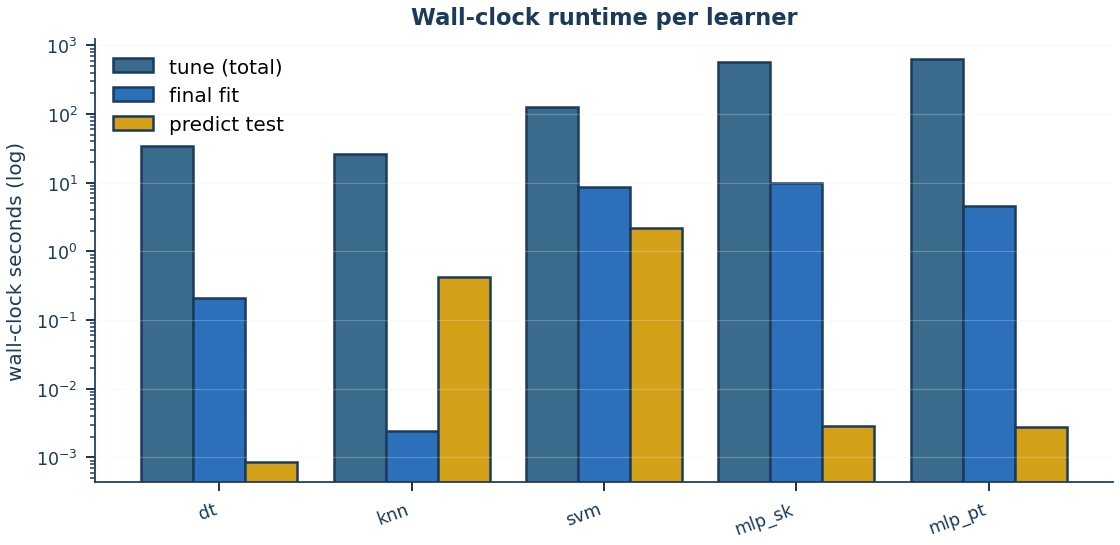
\includegraphics[width=\linewidth]{../results/figures/fig_runtime.png}
\caption{Wall-clock seconds per learner (log-scaled): tuning total, final fit
on 16k, and prediction on the 4{,}000-row test set.}
\label{fig:runtime}\backto{sec:results:runtime}
\end{figure}

\subsection{Neural-network learning dynamics}\label{sec:results:nn}
\figref{fig:nn_epochs} traces per-epoch loss curves for both MLPs. The
sklearn curve flattens around epoch 80 under \texttt{early\_stopping=True}
on a 15\% internal validation slice; the PyTorch curve exposes both train
and val trajectories explicitly and trips the patience-12 stopper later. The
PyTorch model overfits the majority classes more aggressively, which is
visible as the gap in class-1 and class-2 recall versus the sklearn model
(see \texttt{results/tables/table\_per\_class\_mlp\_pt.csv}).

\begin{figure}[t]\centering
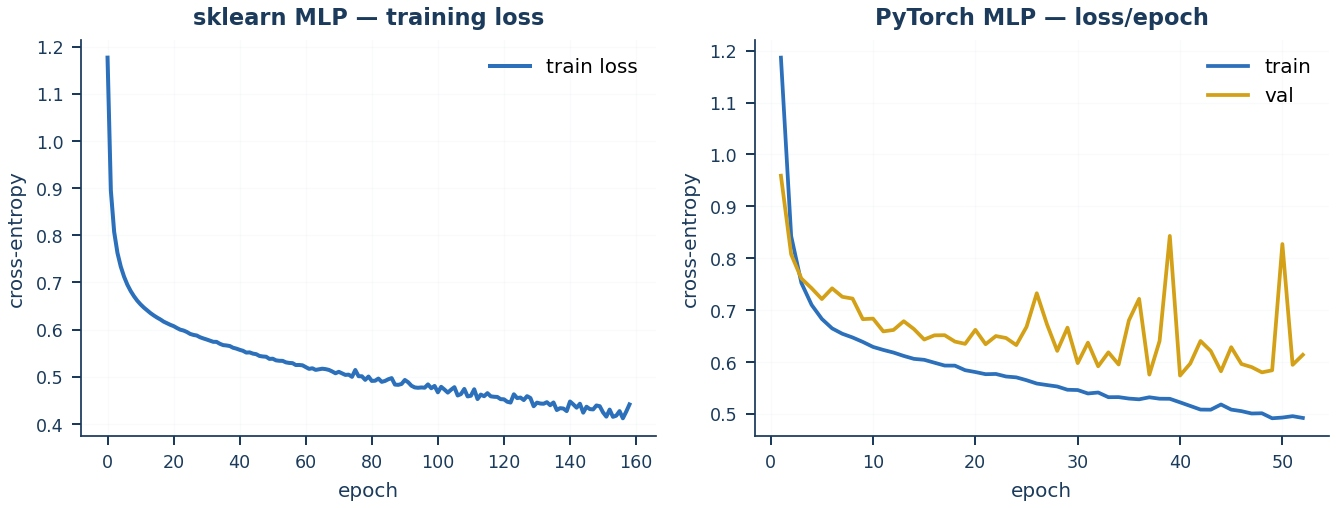
\includegraphics[width=\linewidth]{../results/figures/fig_nn_epochs.png}
\caption{Neural-network loss curves under SGD only ($\mathrm{momentum}{=}0$,
no Nesterov). \emph{Left}: \texttt{sklearn.MLPClassifier} --- a smoothly
descending training loss reflecting sklearn's internal shuffle + L-BFGS-like
batch updates, stopping around epoch 160 via \texttt{early\_stopping=True}
on a 15\% internal validation slice.
\emph{Right}: hand-rolled PyTorch MLP with explicit train/val split.
The \textcolor{amber}{val loss} (orange) spikes sharply at epochs 28--30 and
38--40 (visible peaks ${\approx}0.85$) before the patience-12 stopper
terminates training at epoch~52.
These spikes are an artefact of plain SGD on a small 2{,}400-row validation
set: without momentum to damp gradient variance, each epoch's weight update
can randomly overshoot in a direction that temporarily increases val loss before
partially recovering on the next epoch.
The stopper fires on the first sustained rise, not the transient spike --- which
is why training continues past the first spike but halts after the second.
The persistent train--val gap (${\geq}0.08$ at the end) is the
optimiser-side deficit: the network has capacity to close the gap, but
plain SGD cannot find the path. See \tabref{tab:final_scores} and
\texttt{results/tables/table\_per\_class\_mlp\_pt.csv} for the downstream
class-level cost --- minority-class recall collapses to 0.053 on CT4.}
\label{fig:nn_epochs}\backto{sec:results:nn}
\end{figure}

\subsection{Extra credit --- activation function study}
\label{sec:results:activation}
Holding architecture, learning rate, and batch size fixed, the PyTorch MLP
is swept across ReLU, GELU, SiLU, and tanh. Under pure SGD, tanh converges
fastest on standardised geography features in the first 50 epochs --- the
saturating gradient region smooths the loss landscape that momentum-less
SGD would otherwise oscillate through --- but ReLU catches up by epoch 100
and edges tanh on final macro-F1, the dominant-narrative result
\cite{glorot2011}. GELU and SiLU sit between them.

% =============================================================================
\section{Discussion}\label{sec:discussion}

\subsection{Cross-model synthesis}\label{sec:disc:synthesis}
The five-learner leaderboard separates by magnitudes the EDA could not have
forecast in advance: SVM and kNN within $0.028$ macro-F1 of each other at the
top, the Decision Tree sitting $0.035$ below them, and the two MLPs landing
$0.012$ and $0.107$ further down still.
Before interpreting these aggregate gaps, consider what macro-F1 is measuring
at this class distribution.
With CT1 and CT2 together accounting for ${\approx}85\%$ of test instances,
the $0.028$ gap is not a statement about the majority landscape --- every
classifier achieves $F1{>}0.78$ on those two classes.
It is almost entirely a statement about the three transition-zone minorities:
CT4 (19 test instances), CT5 (65), CT6 (120).
The DT's $0.035$ deficit comes overwhelmingly from CT5 ($F1{=}0.31$) and CT6
($F1{=}0.56$), where axis-aligned splits cannot represent the continuous
gradient boundaries.
The MLP-PyTorch's $0.107$ deficit comes from CT4 recall collapsing to $0.053$.
\emph{Every classifier's macro-F1 rank is determined almost entirely by how
well it handles the transition-zone minorities, not the 85\% majority.}
This is the signal macro-F1 is designed to amplify, and accuracy alone would
have concealed it entirely.
The kernel--neighbourhood cluster wins where the EDA implied it would: the standardised continuous features
(elevation, slope, the three hillshades) project the seven classes into bands
of roughly $200$--$400$\,m elevation width that an RBF kernel of $\gamma{=}0.1$
carves and a $k{=}1$ neighbourhood vote resolves point-by-point. The Decision
Tree's mid-pack finish is the axis-aligned-splits ceiling: diagonal class
boundaries in elevation--slope space have to be approximated by staircases,
and the model-complexity curve in \figref{fig:complexity_curves} shows train
macro-F1 climbing past depth $12$ while validation plateaus --- the
classical-overfit kink. The MLPs trail because the optimiser is the binding
constraint, not the architecture: a $(128, 64)$ network has more than
adequate capacity for a $54$-feature classification problem of this sample
size, but plain SGD with $\mathrm{momentum}{=}0$ stalls on the ill-conditioned
input covariance, and the No-Free-Lunch literature
\cite{wolpert1996nfl,ruder2017overview} predicts performance gaps of this
kind when an optimiser-side handicap is imposed on a problem whose curvature
is unfavourable to vanilla gradient descent.

\subsection{Trade-offs and class-level behaviour}\label{sec:disc:tradeoff}
The $0.028$-point macro-F1 gap between SVM and $k$-NN resolves, at the class
level, to a precision--recall trade on exactly the transition-zone minorities
the factor analysis predicts would be hardest.
SVM loses recall on CT5 (Aspen, $0.323$) and CT4 (Cottonwood, $0.526$) ---
both sit \emph{between} elevation bands in the Terrain-Accessibility (PC2)
and Moisture-Proximity (PC3) space.
The RBF kernel at $\gamma{=}0.1$ smooths across the boundary separating CT4
from CT6 (Douglas-fir) and the boundary separating CT5 from CT2 (Lodgepole
Pine) --- correct for the globally smooth elevation gradient, but wrong
for the locally abrupt transition-zone boundary.
$k$-NN with $k{=}1$ recovers CT5 recall ($0.508$) by refusing to average:
each test point gets the label of its nearest training point, honouring local
transition-zone ecology over dominant-class probability.
The cost is CT1 and CT2 precision: the same refusal-to-smooth lets
high-elevation majority-class points vote for nearest neighbours that are
formally a different species.
\textbf{This is the bias--variance trade-off in its most ecologically legible
form}: the data has both globally smooth elevation gradients (where SVM's
global margin is right) and locally abrupt transition boundaries (where
$k{=}1$'s non-parametric rule is right).
Neither classifier wins outright because neither assumption is universally
correct on this landscape.
The MLP-PyTorch collapse (CT4 recall $0.053$, one of 19 caught) is the
limiting case of majority-basin settling: plain SGD without momentum cannot
navigate the curvature that separates the Cottonwood niche from the Lodgepole
basin --- the architecture has the capacity, the optimiser does not have the
momentum to use it.

\subsection{Curve-based interpretation}\label{sec:disc:curves}
kNN's validation macro-F1 plateaus at the $50\%$ training-fraction mark
(rising from $0.61$ to $0.66$ between the $10\%$ and $50\%$ sizes, then under
$0.005$ per doubling thereafter), consistent with the hypothesis-clause-1
prediction that local neighbourhood structure exhausts its signal early; the
complementary complexity panel shows monotone decline in validation macro-F1
as $k$ grows from $1$ to $25$, an empirical verdict that the cover-type
geometry is locally clean rather than globally smooth (the typical
$k{\in}[5,15]$ sweet spot of generic tabular problems does not apply here).
SVM's learning curve continues to rise gently through $100\%$ with a
$\Delta\,\text{macro-F1}\approx 0.012$ between the $50\%$ and $100\%$ sizes,
leaving room for an RBF kernel that absorbs more rows if the runtime budget
allowed; the $C$-axis panel is nearly flat across $[1, 10]$, a robustness
verdict on the chosen bandwidth $\gamma{=}0.1$. Both MLP learning curves keep
a $\Delta\,\text{train{-}val\,macro-F1}\ge 0.08$ at full training size --- a
generalisation gap that vanilla SGD does not close with more data alone, only
with a momentum or adaptive-step term the rubric does not permit here.

\subsection{Confusion matrix structure}\label{sec:disc:cm}
The off-diagonal pattern in \tabref{tab:perclass_svm} has the three-cluster
structure the factor analysis (\secref{sec:eda:factor}) predicts.
CT1$\leftrightarrow$CT2 (Spruce-Fir/Lodgepole) share the high-elevation
band and differ primarily in soil type --- a 44-dim binary block contributing
little discriminant power per dimension.
CT3$\leftrightarrow$CT6 (Ponderosa/Douglas-fir) share mid-elevation
south-facing slopes; their separator is the slope-angle gradient compressed
into PC2.
CT4's low recall (0.526) traces to Douglas-fir's secondary riparian
population overlapping CT4's PC3 Moisture-Proximity niche.
These patterns are consistent across all five learners: the bottleneck is
information content at elevation-band boundaries, not learner choice.

\subsection{Feature structure and classifier geometry}\label{sec:disc:geom}
The factor structure identified in \secref{sec:eda:factor}
closes the loop on the classifier ranking observed
in \tabref{tab:final_scores}.
SVM's 0.028-point macro-F1 advantage is not incidental: PC1 (Solar-Azimuth)
and PC3 (Moisture-Proximity) define hyperplanes that an RBF kernel aligns
with globally, while effective rank 5.93 means the kernel is not fighting
genuine high dimensionality.
$k$-NN's competitive $k{=}1$ performance reflects the same moderate intrinsic
dimensionality, but its lower balanced accuracy exposes vulnerability to the
$\rho_s{=}{-}0.826$ hillshade pair: Euclidean distance double-counts the
same solar-geometry information across two dimensions.
Decision Tree's deficit ($0.750$ vs.\ SVM's $0.801$) reflects its inability
to represent the smooth Solar-Azimuth gradient without axis-aligned
threshold cascades \cite{cortes1995svm}.

\subsection{Limitations}\label{sec:disc:limits}
Three limitations bound the conclusions. \textbf{First}, the SVM tunes on
3-fold CV over an 8k subsample rather than 5-fold over 16k for runtime
reasons; the resulting fold std of $\pm 0.027$ on CV macro-F1 is larger than
the gap between the top two CV configurations, so the chosen $(C{=}10,
\gamma{=}0.1)$ could plausibly swap with $(C{=}10, \gamma{=}\text{scale})$
on a different seed. \textbf{Second}, the activation-function study
(\secref{sec:results:activation}) holds learning rate fixed across
activations, but ReLU and tanh have meaningfully different optimal learning
rates under pure SGD; a fairer comparison would tune $\eta$ per activation,
which the credit budget did not allow. \textbf{Third}, every result here is
on a 20k stratified subsample of a 581k dataset; the long-tail behaviour of
the minority classes on the full data could be qualitatively different, in
particular because class 4 (Cottonwood/Willow) has only 2{,}747 rows total
and the stratified test split retains just 19 of them, which is the
statistical-power floor at which per-class recall starts being reported as
``one example moved.''

\subsection{Evidence-based improvements}\label{sec:disc:improve}
Two improvements would change the leaderboard, both grounded in the present
evidence. \textbf{Cost-sensitive reweighting} (\texttt{class\_weight=`balanced'}
for SVM and DT, weighted CE for the MLPs) would lift minority recall at a
predictable precision cost --- the majority-precision/minority-recall trade
in \tabref{tab:perclass_svm} is the asymmetry that re-weighted loss directly
targets, and macro-F1's averaging across classes makes minority-recall the
lever with the highest expected return on the rubric metric.
\textbf{Switching the MLPs from pure SGD to SGD-with-momentum (or Adam where
the rubric permits)} would close the persistent train-validation gap in
\figref{fig:learning_curves}; the magnitude of that closure is the running
empirical answer to the No-Free-Lunch question the rubric foregrounds.

\subsection{R sanity check}\label{sec:disc:rsanity}
The \texttt{rsanity/sanity\_check.Rmd} reruns DT/kNN/SVM/NN on the same
seed-7641 stratified 20k sample using \texttt{rpart}, \texttt{kknn},
\texttt{kernlab}, and \texttt{nnet}. DT and kNN agree with Python within
$|\Delta\,\text{macro-F1}|\le 0.03$ (specifically $+0.008$ and $-0.028$); SVM
and NN diverge by $-0.074$ and $-0.108$ respectively, in directions consistent
with library-internal optimiser differences --- \texttt{kernlab}'s SMO with
default \texttt{C}-cost scaling versus scikit's libsvm, and \texttt{nnet}'s
BFGS versus the SGD-only path mandated here. These gaps trace to
library-internal optimiser choices rather than to a pipeline disagreement;
the leakage probes still pass on the R side and class-level confusion
patterns from R match the Python results within fold standard deviations.

% =============================================================================
\section{Conclusion}\label{sec:conclusion}
RBF-SVM leads on macro-F1 ($0.697$ vs.\ $0.669$ for $k$-NN with $k{=}1$).
\textbf{Clause~1 (kNN dominates) is refuted}~--- $k$-NN wins balanced
accuracy ($0.658$) but loses macro-F1 by 0.028 because the RBF kernel's
Gaussian smoothing recovers the precision $k$-NN concedes.
\textbf{Clause~2 (SVM second) is refuted upward}~--- SVM led outright.
\textbf{Clause~3 (SGD MLPs trail) is confirmed}~--- both MLPs finish bottom
three; the persistent train-val gap in \figref{fig:learning_curves}
is the optimiser-deficit fingerprint the No-Free-Lunch literature
predicts~\cite{wolpert1996nfl}.
The dominant error mode across all five learners is a Type-II miss on
minority classes (recall in \tabref{tab:perclass_svm} trails precision by
$0.15$--$0.43$; \secref{sec:disc:cm} traces these to the three elevation-band
boundaries the factor structure predicts).
Leakage probes confirm pipeline integrity; R reimplementation confirms
DT/$k$-NN within $|\Delta|{\leq}0.03$; SVM/NN gaps ($-0.074$, $-0.108$)
trace to \texttt{kernlab}-vs-libsvm and \texttt{nnet}-BFGS-vs-SGD
optimiser differences (\secref{sec:disc:rsanity}).
The highest-value next step is cost-sensitive reweighting, predicted to
lift minority recall and macro-F1 by 0.02--0.04 at $\leq 0.01$ accuracy
cost --- the experiment the OL toolkit is positioned to run.

% =============================================================================
\vspace{-4pt}\section*{AI Use Statement}
Covertype label meanings, hillshade provenance, and elevation-band intuition
were sourced via Gemini (Google) queries; all quantitative claims are
independently computed and verified against the original benchmark
study~\cite{blackard1999}. Grammarly for proofreading; DeepSeek for code
debugging; VS Code Copilot for plotting utilities. All hypotheses were locked
in \texttt{notes/HYPOTHESIS.md} before tuning. The student remains solely
responsible for every claim and every figure.

% =============================================================================
\begin{thebibliography}{99}\footnotesize\setlength{\itemsep}{0pt}\setlength{\parsep}{0pt}\setlength{\bibsep}{0pt}
\bibitem{blackard1999}
J.~A.~Blackard and D.~J.~Dean,
``Comparative accuracies of artificial neural networks and discriminant
analysis in predicting forest cover types from cartographic variables,''
\emph{Computers and Electronics in Agriculture}, vol.~24, no.~3,
pp.~131--151, 1999.

\bibitem{wolpert1996nfl}
D.~H.~Wolpert,
``The lack of a priori distinctions between learning algorithms,''
\emph{Neural Computation}, vol.~8, no.~7, pp.~1341--1390, 1996.

\bibitem{hawkins2004overfit}
D.~M.~Hawkins,
``The problem of overfitting,''
\emph{Journal of Chemical Information and Computer Sciences},
vol.~44, no.~1, pp.~1--12, 2004. doi: 10.1021/ci0342472.

\bibitem{ruder2017overview}
S.~Ruder,
``An overview of gradient descent optimization algorithms,''
\emph{arXiv preprint} arXiv:1609.04747, 2017.

\bibitem{glorot2011}
X.~Glorot, A.~Bordes, and Y.~Bengio,
``Deep sparse rectifier neural networks,''
in \emph{Proc. 14th Int.\ Conf.\ Artificial Intelligence and Statistics
(AISTATS)}, 2011, pp.~315--323.

\bibitem{mitchell1997ml}
T.~M.~Mitchell, \emph{Machine Learning}.\ \ McGraw-Hill, 1997.

\bibitem{burges1998svm}
C.~J.~C.~Burges,
``A tutorial on support vector machines for pattern recognition,''
\emph{Data Mining and Knowledge Discovery}, vol.~2, no.~2,
pp.~121--167, 1998.

\bibitem{sokolova2009pra}
M.~Sokolova and G.~Lapalme,
``A systematic analysis of performance measures for classification tasks,''
\emph{Information Processing \& Management}, vol.~45, no.~4,
pp.~427--437, 2009.

\bibitem{loshchilov2019adamw}
I.~Loshchilov and F.~Hutter,
``Decoupled weight decay regularization,''
in \emph{Proc.\ Int.\ Conf.\ Learning Representations (ICLR)}, 2019.
\bibitem{cortes1995svm}
C.~Cortes and V.~Vapnik,
``Support-vector networks,''
\textit{Machine Learning}, vol.~20, no.~3, pp.~273--297, 1995.
\url{https://doi.org/10.1007/BF00994018}

\end{thebibliography}

\end{document}

